% NeurAps — Insight 2.0 Grand Finale (Beamer)
% Build: pdflatex neuraps_finale.tex  (run twice)
\documentclass[aspectratio=169,10pt]{beamer}

\usepackage[T1]{fontenc}
\usepackage{libertine}   % Linux Libertine serif + Biolinum sans
% mono: default lmodern typewriter
\usepackage{booktabs}
\usepackage{tikz}
\usetikzlibrary{positioning}

% ---------- palette ----------
\definecolor{navy}{HTML}{1F3A5F}
\definecolor{burg}{HTML}{8C2F2F}
\definecolor{ink}{HTML}{1A1A1A}
\definecolor{mutedgray}{HTML}{555F66}
\definecolor{lightbg}{HTML}{F2F5F8}
\definecolor{ruleline}{HTML}{D6DBE0}

% ---------- theme (hand-built, metropolis-inspired) ----------
\usetheme{default}
\definecolor{paper}{HTML}{FCFCFA}
\definecolor{navyfaint}{HTML}{2C4A73}
\setbeamercolor{background canvas}{bg=paper}
\setbeamercolor{structure}{fg=navy}
\setbeamercolor{frametitle}{fg=navy,bg=paper}
\setbeamercolor{title}{fg=white}
\setbeamercolor{normal text}{fg=ink}
\setbeamercolor{alerted text}{fg=burg}
\setbeamercolor{block title}{fg=paper,bg=navy}
\setbeamercolor{block body}{fg=ink,bg=lightbg}
\setbeamercolor{block title alerted}{fg=paper,bg=burg}
\setbeamercolor{block body alerted}{fg=ink,bg=lightbg}
\setbeamertemplate{navigation symbols}{}
\setbeamertemplate{blocks}[rounded]
\setbeamertemplate{itemize item}{\tikz{\fill[burg] (0,0) rectangle (0.55ex,0.55ex);}}
\setbeamertemplate{itemize subitem}{\tikz{\draw[navy,thick] (0,0) rectangle (0.5ex,0.5ex);}}
\setbeamerfont{frametitle}{series=\bfseries,size=\LARGE}
\setbeamersize{text margin left=1.05cm,text margin right=1.05cm}

% frame title: bold navy with a short burgundy underline
\setbeamertemplate{frametitle}{%
  \vspace{0.55cm}%
  {\usebeamerfont{frametitle}\usebeamercolor[fg]{frametitle}\insertframetitle}\par
  \vspace{0.12cm}{\color{burg}\rule{1.35cm}{2.6pt}}\par\vspace{0.1cm}}

% footline: metropolis-style progress bar + label + page
\setbeamertemplate{footline}{%
  \begin{tikzpicture}[baseline]
    \fill[ruleline] (0,0) rectangle (\paperwidth,0.55mm);
    \pgfmathsetmacro{\prog}{\insertframenumber/\inserttotalframenumber*\paperwidth/1cm}
    \fill[burg] (0,0) rectangle (\prog cm,0.55mm);
  \end{tikzpicture}\par\vspace{1.4pt}%
  \hspace{1.05cm}{\tiny\color{mutedgray}Insight 2.0 --- Datathon 2026 \;·\; Team NeurAps}%
  \hfill{\tiny\color{mutedgray}\insertframenumber\,/\,\inserttotalframenumber}\hspace{1.05cm}\vspace{3.5pt}}

% section page: navy field, giant ghost number, burgundy tick
\setbeamertemplate{section page}{%
  \begin{tikzpicture}[remember picture,overlay]
    \fill[navy] (current page.south west) rectangle (current page.north east);
    \node[anchor=south east,color=navyfaint,font=\fontsize{130}{130}\selectfont\bfseries,
          inner sep=0pt,opacity=0.85] at ([xshift=-0.4cm,yshift=0.2cm]current page.south east)
          {\insertsectionnumber};
    \node[anchor=west,color=white,font=\huge\bfseries,text width=0.8\paperwidth,align=left]
          at ([xshift=1.2cm,yshift=0.3cm]current page.west) {\insertsection};
    \draw[burg,line width=3pt] ([xshift=1.2cm,yshift=1.35cm]current page.west) -- ++(1.35,0);
    \node[anchor=west,color=ruleline,font=\small]
          at ([xshift=1.2cm,yshift=1.85cm]current page.west) {Section \insertsectionnumber};
  \end{tikzpicture}}
\AtBeginSection[]{\begin{frame}[plain]\sectionpage\end{frame}}

\title{Survival Classification of Lung-Cancer Patients:\\
       A Cross-Validation-First Approach on SEER Registry Data}
\author{\textbf{Team NeurAps}}
\institute{Insight 2.0 --- Grand Finale \;·\; IASDS Students' Club, University of Dhaka}
\date{5 September 2026}

\newcommand{\stat}[2]{{\color{navy}\ttfamily\bfseries\large #1}\\{\scriptsize\color{mutedgray}#2}}
\newcommand{\astat}[2]{{\color{burg}\ttfamily\bfseries\large #1}\\{\scriptsize\color{mutedgray}#2}}

\begin{document}

% ---------- 1 title ----------
\begin{frame}[plain]
  \begin{tikzpicture}[remember picture,overlay]
    \fill[navy] (current page.south west) rectangle (current page.north east);
    \fill[burg] ([yshift=-0.0cm]current page.north west) rectangle
                ([yshift=-0.16cm]current page.north east);
    \node[anchor=west,color=ruleline,font=\footnotesize\ttfamily]
      at ([xshift=1.2cm,yshift=-1.5cm]current page.north west)
      {INSIGHT 2.0 --- GRAND FINALE \;·\; IASDS STUDENTS' CLUB, UNIVERSITY OF DHAKA};
    \node[anchor=west,color=white,font=\LARGE\bfseries,text width=0.86\paperwidth,align=left]
      at ([xshift=1.2cm,yshift=0.75cm]current page.west)
      {Survival Classification of Lung-Cancer Patients:\\[4pt]
       A Cross-Validation-First Approach\\[4pt]
       on SEER Registry Data};
    \draw[burg,line width=3pt] ([xshift=1.2cm,yshift=2.1cm]current page.west) -- ++(1.35,0);
    \node[anchor=west,color=ruleline,font=\large]
      at ([xshift=1.2cm,yshift=-0.75cm]current page.west)
      {\textbf{\color{white}Team NeurAps} \;·\; 5 September 2026};
    % stats row
    \node[anchor=west,color=white,font=\ttfamily\bfseries\large]
      at ([xshift=1.2cm,yshift=-2.15cm]current page.west) {0.880410};
    \node[anchor=west,color=ruleline,font=\scriptsize]
      at ([xshift=1.2cm,yshift=-2.65cm]current page.west) {private weighted F1};
    \node[anchor=west,color=white,font=\ttfamily\bfseries\large]
      at ([xshift=5.4cm,yshift=-2.15cm]current page.west) {4th / 79};
    \node[anchor=west,color=ruleline,font=\scriptsize]
      at ([xshift=5.4cm,yshift=-2.65cm]current page.west) {final private rank};
  \end{tikzpicture}
\end{frame}

% ---------- 2 outline: the 8 required components ----------
\begin{frame}{Outline --- covering all eight required components}
  \small
  \begin{enumerate}
    \item \textbf{Summary of Our Work} --- overall approach and headline result
    \item \textbf{Exploratory Data Analysis} --- imbalance, the diagnosis-year effect, data quality
    \item \textbf{Feature Selection} --- what we kept, what we audited, and why
    \item \textbf{Feature Engineering} --- features created and transformed, with rationale
    \item \textbf{Model Selection} --- models considered and the reasoning behind choices
    \item \textbf{Model Evaluation} --- validation design and metric-faithful evaluation
    \item \textbf{Model Comparison} --- head-to-head performance of every model tried
    \item \textbf{Best Findings} --- key insights and final conclusions
  \end{enumerate}
\end{frame}

\section{Summary of Our Work}

\begin{frame}{Problem statement and result}
  Given SEER cancer-registry records of lung-cancer patients (all primary sites C34.x),
  predict \texttt{vital\_status} $\in$ \{Alive, Dead\}. Metric: \alert{weighted F1}
  on a hidden test set (40\% public / 60\% private).
  \vspace{6pt}
  \begin{columns}
    \column{.25\textwidth}\centering \stat{24{,}000}{training records}
    \column{.25\textwidth}\centering \stat{36{,}000}{test records (1.5$\times$)}
    \column{.25\textwidth}\centering \stat{36}{clinical features}
    \column{.25\textwidth}\centering \stat{6/day}{submission budget}
  \end{columns}
  \vspace{8pt}
  \begin{block}{Our approach in one sentence}
    Engineered clinical features $\rightarrow$ a blend of three gradient-boosted tree models,
    trained twice (plain, then with pseudo-labelled test rows), mixed with 5\% each of
    RandomForest, ExtraTrees and an MLP, thresholded at 0.575 --- every decision gated by
    honest out-of-fold cross-validation.
  \end{block}
\end{frame}

\section{Exploratory Data Analysis}

\begin{frame}{The target is heavily imbalanced}
  \begin{columns}
    \column{.4\textwidth}\centering \stat{83.0\%}{of patients are Dead}\\[10pt] \astat{17.0\%}{are Alive}
    \column{.6\textwidth}
    \textbf{Why this matters for weighted F1:}
    \begin{itemize}
      \item An all-Dead baseline reaches 0.907 Dead-class F1 but only $\sim$0.75 weighted F1 ---
            the minority class carries decisive weight.
      \item The decision threshold becomes a first-class model parameter.
      \item Stratified resampling is mandatory in cross-validation.
    \end{itemize}
  \end{columns}
\end{frame}

\begin{frame}{The dominant covariate: year of diagnosis}
  \begin{columns}
    \column{.6\textwidth}
    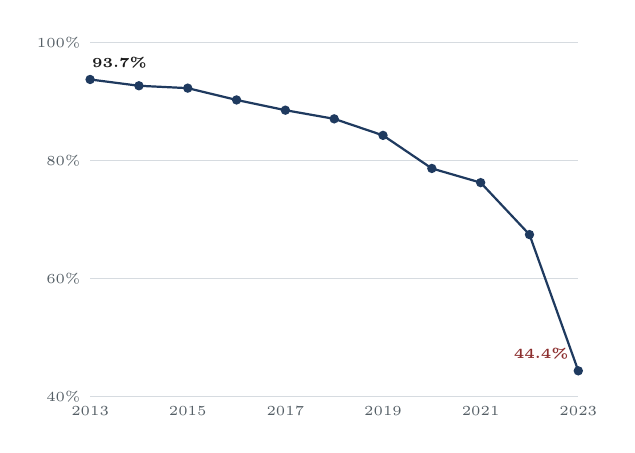
\begin{tikzpicture}[x=0.62cm,y=1cm]
      % grid + axis labels (death rate 40--100%)
      \foreach \yy/\lab in {0/40, 1.5/60, 3.0/80, 4.5/100}{
        \draw[ruleline] (0,\yy) -- (10,\yy);
        \node[left,font=\tiny,color=mutedgray] at (0,\yy) {\lab\%};}
      \foreach \xx/\lab in {0/2013, 2/2015, 4/2017, 6/2019, 8/2021, 10/2023}
        \node[below,font=\tiny,color=mutedgray] at (\xx,0) {\lab};
      \draw[navy,thick]
        (0,4.03)--(1,3.95)--(2,3.92)--(3,3.77)--(4,3.64)--(5,3.53)
        --(6,3.32)--(7,2.90)--(8,2.72)--(9,2.06)--(10,0.33);
      \foreach \p in {(0,4.03),(1,3.95),(2,3.92),(3,3.77),(4,3.64),(5,3.53),
                      (6,3.32),(7,2.90),(8,2.72),(9,2.06),(10,0.33)}
        \fill[navy] \p circle (1.7pt);
      \node[above,font=\tiny\bfseries,color=ink] at (0.6,4.05) {93.7\%};
      \node[left,font=\tiny\bfseries,color=burg] at (10,0.55) {44.4\%};
    \end{tikzpicture}
    \column{.4\textwidth}\small
    \alert{93.7\% $\rightarrow$ 44.4\%} --- a right-censoring artifact: recent patients
    have not been followed long enough to die.
    \begin{itemize}\scriptsize
      \item Train/test share the year distribution $\Rightarrow$ random split
            $\Rightarrow$ StratifiedKFold is the honest CV scheme.
      \item Errors concentrate in recent years (23\% in 2023 vs 6\% in 2013).
      \item \texttt{years\_since\_dx} becomes a first-class feature.
    \end{itemize}
  \end{columns}
\end{frame}

\begin{frame}{Data quality: sentinel codes, not NaN}
  \begin{columns}[t]
    \column{.5\textwidth}
    \begin{block}{Coded missingness}\scriptsize
      Tumor size uses 999 / ``Blank(s)'' / ``Unknown''; one surgery-scope column is 66.5\% null
      by era definition. Decoded to numerics + explicit missingness flags.
    \end{block}
    \begin{block}{Era-dependent columns}\scriptsize
      Size and staging switch coding systems across eras; we coalesce into single
      best-available features instead of discarding either era.
    \end{block}
    \column{.5\textwidth}
    \begin{block}{Leakage checks}\scriptsize
      No duplicate IDs; row order uninformative; every high-power feature audited individually.
    \end{block}
    \begin{block}{Informative categories}\scriptsize
      ``Death certificate only'' and ``died prior to recommended surgery'' directly signal
      the outcome, appear in both splits --- legitimate, powerful features.
    \end{block}
  \end{columns}
\end{frame}

\section{Features: Selection \& Engineering}

\begin{frame}{Feature selection: what we kept, and why}
  Starting point: all 36 provided features. Final model: all 36 + $\sim$15 engineered.
  Retention was a \textbf{tested} decision, not a default.
  \begin{itemize}
    \item \textbf{No hard filtering:} GBDTs select implicitly --- uninformative features are never
          chosen for splits. Dropping low-importance features worsened CV every time we tried.
    \item \textbf{Importance-ranked signal:} surgery-decision codes, summary stage / TNM,
          year of diagnosis, age, tumor size, metastasis flags --- clinically coherent.
    \item \textbf{Leakage audit as selection:} every strong feature individually audited; all passed.
    \item \textbf{No shift-based drops:} train/test distributions align; nothing sacrificed for stability.
  \end{itemize}
\end{frame}

\begin{frame}{Feature engineering}
  \scriptsize
  \begin{tabular}{@{}p{3.4cm}p{9.2cm}@{}}
    \toprule
    \textbf{Feature} & \textbf{Construction and justification}\\
    \midrule
    \texttt{t/n/m\_ord} & T/N/M staging mapped to ordered scales --- staging is clinically ordinal\\
    \texttt{tnm\_sum} & composite stage score, metastasis double-weighted\\
    \texttt{tumor\_size\_best} & three era-coded columns parsed and coalesced + missing flags\\
    \texttt{mets\_count} & count of metastatic sites --- graded severity signal\\
    \texttt{nodes\_ratio} & positive/examined nodes --- normalizes surgical thoroughness\\
    treatment flags & surgery, radiation, death-certificate-only --- physician prognosis signal\\
    \texttt{years\_since\_dx} & the censoring proxy (see EDA)\\
    \bottomrule
  \end{tabular}
  \vspace{5pt}\par\tiny\color{mutedgray}
  Deliberately avoided: fold-external target encoding, anything fitted on test, AutoML.
\end{frame}

\section{Model Selection \& Evaluation}

\begin{frame}{Model selection: why three GBDTs}
  \begin{itemize}
    \item \textbf{LightGBM} --- leaf-wise growth, histogram splits, native categoricals: the workhorse.
    \item \textbf{XGBoost} --- depth-wise growth, second-order gradients: same family,
          \emph{different mistakes}.
    \item \textbf{CatBoost} --- ordered target statistics: built for 114-level histology codes.
    \item Their OOF correlation is $\sim$0.97 --- but the 3\% disagreement sits exactly on the
          uncertain rows where F1 is decided; the blend beats every member.
    \item \textbf{Diversity mixture:} RandomForest, ExtraTrees, MLP at 5\% each ---
          weaker solo, decorrelated errors; verified $+0.0006$ by split-half testing.
    \item \textbf{Why not deep learning?} Measured, not assumed: MLP 0.874 solo,
          TabPFN correlated 0.98 with the blend. At 24k rows, trees win.
  \end{itemize}
\end{frame}

\begin{frame}{The final architecture}
  \centering
  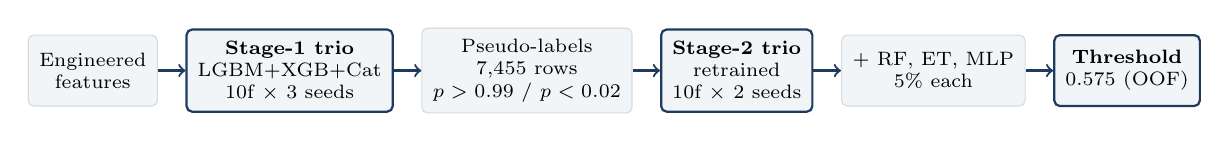
\begin{tikzpicture}[
    node distance=3.5mm,
    stage/.style={draw=navy,thick,fill=lightbg,rounded corners=2pt,align=center,
                  font=\scriptsize,minimum height=9mm,inner sep=4pt},
    plain/.style={draw=ruleline,fill=lightbg,rounded corners=2pt,align=center,
                  font=\scriptsize,minimum height=9mm,inner sep=4pt},
    arr/.style={->,thick,navy}]
    \node[plain] (f) {Engineered\\features};
    \node[stage,right=of f] (s1) {\textbf{Stage-1 trio}\\LGBM+XGB+Cat\\10f $\times$ 3 seeds};
    \node[plain,right=of s1] (pl) {Pseudo-labels\\7{,}455 rows\\$p>0.99$ / $p<0.02$};
    \node[stage,right=of pl] (s2) {\textbf{Stage-2 trio}\\retrained\\10f $\times$ 2 seeds};
    \node[plain,right=of s2] (dv) {+ RF, ET, MLP\\5\% each};
    \node[stage,right=of dv] (th) {\textbf{Threshold}\\0.575 (OOF)};
    \draw[arr] (f)--(s1); \draw[arr] (s1)--(pl); \draw[arr] (pl)--(s2);
    \draw[arr] (s2)--(dv); \draw[arr] (dv)--(th);
  \end{tikzpicture}
  \vspace{10pt}
  \begin{block}{Model evaluation protocol (identical for every candidate)}
    Stratified 10-fold out-of-fold weighted F1 with tuned threshold; multiple seeds;
    honest split-half verification for every \emph{selected} quantity;
    the public leaderboard used only for controlled single-variable probes.
  \end{block}
\end{frame}

\begin{frame}{Pseudo-labelling: our biggest win, done honestly}
  \begin{itemize}
    \item The test set is 1.5$\times$ the training data: 36{,}000 unlabelled in-distribution rows.
    \item Only extreme confidences cross over ($p>0.99 \rightarrow$ Dead, $p<0.02 \rightarrow$ Alive):
          7{,}455 rows, expected label noise 1--2\%.
    \item \alert{CV integrity:} pseudo-rows join only the training side of each fold;
          evaluation stays on original labelled rows --- the estimate remains unbiased.
    \item Extensions tested and rejected: wider bands (no gain), a second round (no gain).
  \end{itemize}
\end{frame}

\section{Model Comparison \& Experiments}

\begin{frame}{Model comparison: every model, head to head}
  \scriptsize
  \begin{tabular}{@{}lll@{}}
    \toprule
    \textbf{Model / configuration} & \textbf{OOF wF1} & \textbf{Role}\\
    \midrule
    ExtraTrees (800 trees)            & 0.87266 & 5\% of final mixture\\
    Logistic regression (one-hot)     & 0.87326 & rejected --- diversity candidate\\
    MLP 128$\times$64                 & 0.87393 & 5\% of final mixture\\
    RandomForest (800 trees)          & 0.87432 & 5\% of final mixture\\
    HistGradientBoosting              & 0.87502 & rejected\\
    TabPFN (foundation model)         & 0.87644 & rejected --- 0.98 corr.\ with blend\\
    LightGBM (single, default)        & 0.87646 & baseline reference\\
    CatBoost (10f $\times$ 3 seeds)   & 0.87871 & blend member\\
    XGBoost (10f $\times$ 3 seeds)    & 0.87885 & blend member\\
    LightGBM, focal loss $\gamma{=}1$ & 0.87982 & best single --- gain overlapped blend\\
    GBM trio + pseudo-labels          & 0.87965 & stage-2 core\\
    \textbf{Final: + RF/ET/MLP mixture} & \textbf{0.87996} & \textbf{submitted --- private 0.880410}\\
    \bottomrule
  \end{tabular}
\end{frame}

\begin{frame}{Negative results: rejected with evidence}
  \begin{columns}[t]
    \column{.5\textwidth}
    \begin{alertblock}{Aggressive Optuna tuning}\scriptsize
      $+0.002$ OOF, $-0.0005$ leaderboard --- CV overfitting via 40 trials on the same folds.
      Proven with a controlled probe; tuning stopped there.
    \end{alertblock}
    \begin{alertblock}{Soft-label distillation}\scriptsize
      $+0.001$ CV was the teacher leaking validation information through soft labels;
      leaderboard flat. The CV gain was provably spurious.
    \end{alertblock}
    \column{.5\textwidth}
    \begin{alertblock}{Per-year thresholds}\scriptsize
      In-sample $+0.001$; \emph{worse} under split-half verification ---
      eleven fragmented optimizations, eleven chances to fit noise.
    \end{alertblock}
    \begin{alertblock}{More model families}\scriptsize
      Everything correlated $\ge 0.97$ with the blend. The dataset's signal saturates
      near OOF $\approx 0.880$ --- a measured ceiling.
    \end{alertblock}
  \end{columns}
\end{frame}

\begin{frame}{The decisive call: public vs.\ private}
  \begin{columns}
    \column{.55\textwidth}
    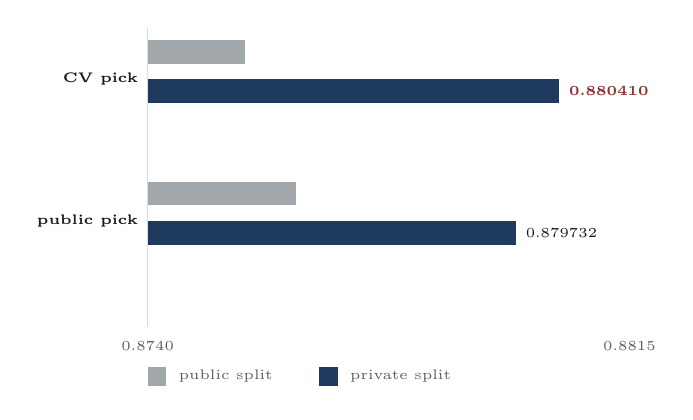
\begin{tikzpicture}[x=0.68cm,y=1cm]
      % horizontal bars, scale 0.874 -> 0.8815 over 9 units
      \draw[ruleline] (0,-0.4) -- (0,3.4);
      \node[below,font=\tiny,color=mutedgray] at (0,-0.45) {0.8740};
      \node[below,font=\tiny,color=mutedgray] at (9,-0.45) {0.8815};
      % CV pick (scored): public 0.875506 -> 1.81, private 0.880410 -> 7.69
      \node[left,font=\tiny\bfseries,color=ink] at (0,2.75) {CV pick};
      \fill[mutedgray!55] (0,2.95) rectangle (1.81,3.25);
      \fill[navy]         (0,2.45) rectangle (7.69,2.75);
      \node[right,font=\tiny\bfseries,color=burg] at (7.69,2.6) {0.880410};
      % public pick: public 0.876311 -> 2.77, private 0.879732 -> 6.88
      \node[left,font=\tiny\bfseries,color=ink] at (0,0.95) {public pick};
      \fill[mutedgray!55] (0,1.15) rectangle (2.77,1.45);
      \fill[navy]         (0,0.65) rectangle (6.88,0.95);
      \node[right,font=\tiny,color=ink] at (6.88,0.8) {0.879732};
      % legend
      \fill[mutedgray!55] (0,-1.15) rectangle (0.35,-0.9);
      \node[right,font=\tiny,color=mutedgray] at (0.4,-1.02) {public split};
      \fill[navy] (3.2,-1.15) rectangle (3.55,-0.9);
      \node[right,font=\tiny,color=mutedgray] at (3.6,-1.02) {private split};
    \end{tikzpicture}
    \column{.45\textwidth}\small
    \begin{itemize}\scriptsize
      \item Measured: public deltas $<0.0008$ between our submissions were split noise.
      \item Strategy: one final by public score, one by honest CV.
      \item The CV pick --- \emph{punished} by the public board --- scored
            \alert{0.880410} and delivered 4th.
      \item Auto-selection would have finished $\approx$ 9th.
    \end{itemize}
  \end{columns}
\end{frame}

\section{Best Findings}

\begin{frame}{Final results: the CV estimate was the truth}
  \begin{columns}
    \column{.33\textwidth}\centering \stat{0.87996}{OOF forecast (pre-reveal)}
    \column{.33\textwidth}\centering \astat{0.880410}{private result}
    \column{.33\textwidth}\centering \stat{0.0004}{forecast error}
  \end{columns}
  \vspace{14pt}
  \begin{columns}
    \column{.5\textwidth}\centering \stat{30th $\rightarrow$ 4th}{public rank $\rightarrow$ private rank}
    \column{.5\textwidth}\centering \stat{0.000075}{gap to 3rd ($\approx$ 3 patients of 36{,}000)}
  \end{columns}
  \vspace{10pt}\centering\scriptsize\color{mutedgray}
  Several teams above us on the public board fell out of the private top ten ---
  the signature of public-split overfitting.
\end{frame}

\begin{frame}{Four principles that decided this result}
  \begin{enumerate}
    \item \textbf{Identify the exact metric before modelling.} One OOF sweep revealed weighted F1
          and made the threshold a model parameter.
    \item \textbf{Trust out-of-fold CV; treat the public leaderboard as an instrument.}
          Controlled single-variable probes; never chase it.
    \item \textbf{Verify every gain adversarially.} Split-half testing killed three
          seductive ``improvements'' that were bias or leakage.
    \item \textbf{Log everything --- negative results compound.} A complete experiment ledger made
          the endgame a calculation, not a gamble.
  \end{enumerate}
\end{frame}

\begin{frame}{Limitations \& future work}
  \begin{itemize}
    \item \textbf{Censoring is implicit, not modelled} --- a survival-analysis formulation
          (Cox PH, discrete-time hazard, boosted survival trees) is the statistically
          superior next step.
    \item \textbf{Per-era probability calibration} could sharpen the single global threshold.
    \item \textbf{Interpretability:} SHAP attribution of the final ensemble remains future work.
    \item \textbf{Compute-bounded:} four days on one laptop bounded ensemble size and search depth.
  \end{itemize}
  \vspace{6pt}\scriptsize\color{mutedgray}
  Tools: Python 3.12, pandas, scikit-learn, LightGBM, XGBoost, CatBoost, Optuna.
  All seeds fixed; the submitted notebook re-runs end-to-end in $\approx$ 1 hour and
  regenerates our selected predictions exactly. No external data used.
\end{frame}

% ---------- thanks ----------
\begin{frame}[plain]
  \begin{tikzpicture}[remember picture,overlay]
    \fill[navy] (current page.south west) rectangle (current page.north east);
  \end{tikzpicture}
  \vspace{2.6cm}
  {\color{white}\Huge\bfseries Thank you.}\\[10pt]
  {\color{ruleline}\large Questions welcome --- every claim is reproducible from our
   notebook and experiment ledger.}\\[22pt]
  {\color{ruleline}\ttfamily\small Team NeurAps \;·\; Insight 2.0 --- Datathon 2026 \;·\;
   private weighted F1 0.880410 (4th of 79)}
\end{frame}

\end{document}
